\section{Box-office Predicting}
\label{sec:predict}
\subsection{Premiere week box-office predicting}
\subsection{Phased Box-office Predicting}
\begin{figure}[!htbp]
\centering
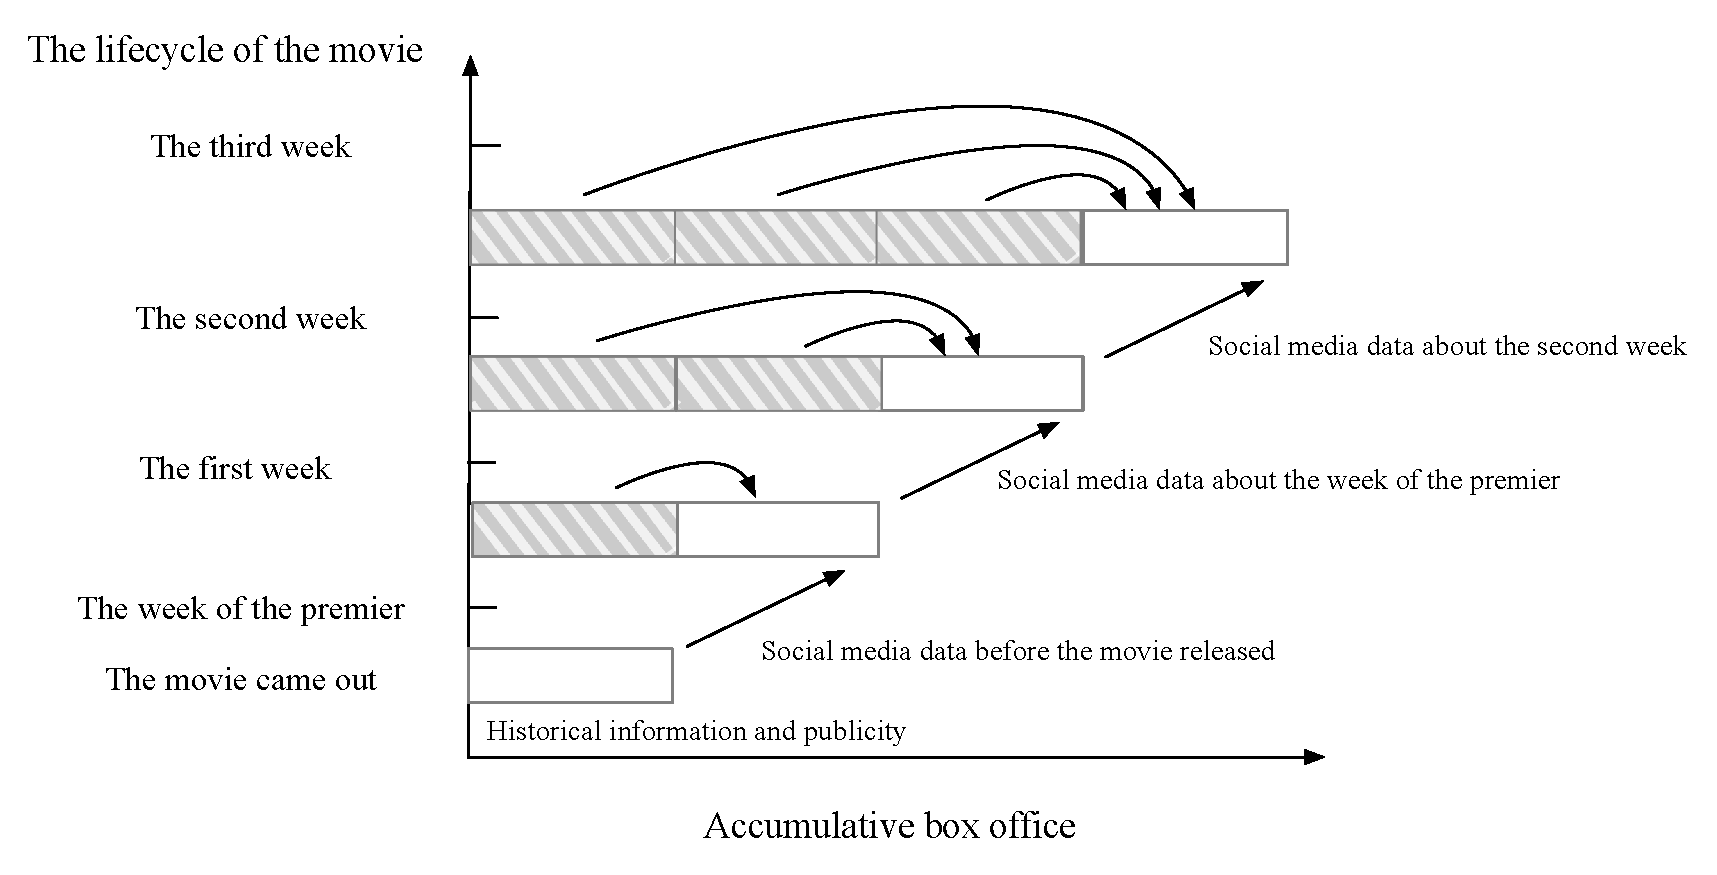
\includegraphics[width=0.8\columnwidth]{boxpredict.eps}
\caption{Multi-stage box office prediction model}
\label{fig:mhin}
\end{figure}
In the past prediction of box office, we usually only forecast the overall box office, but often ignored the movie's influence on movie box office due to the audience's attitude. Such as "wolf 2", the movie box office to be among the world's top 100, because in the release process, because the audience warmly, attracted the audience is not the original film (film series the fans, fans, like the kind of audience) to watch a movie, which leads to the box office continued to rise however, the traditional model is unable to capture this phenomenon. Therefore, from the pre launch to the 1 months after the release, we set up the box office prediction model with the weekly variation of the weekly release to predict the box office for the first week, the box office for second weeks, the third week box office and the box office at the fourth week.\\
\begin{table}[!htb]
  \centering
\begin{tabular}{|c|c|}
\hline
Symbol&Description\\
\hline
sc&\tabincell{c}{The mean bos of well-known \\ actors and directors}\\
\hline
gsc&\tabincell{c}{The mean wms of well-known \\ actors and directors}\\
\hline
std&\tabincell{c}{The variance bos of well-known \\ actors and directors}\\
\hline
gstd&\tabincell{c}{The variance wms of well-known \\ actors and directors}\\
\hline
$weibo_i$&\tabincell{c}{The ratio of creative comments and \\ all comments until the $ith$ week}\\
\hline
$week_i$&\tabincell{c}{The box office in the $ith$ week}\\
\hline
\end{tabular}
  \caption{Features}
\end{table}
